\chapter{Strängars rörelse i vätskor}

%\subsubsection{Strängrörelser inom cellen}
Aktinfilament är polymerer vilka utgör en viktig byggsten för cellens cytoskelett och transportväg för motorprotein vilka formar och bidrar till cellens utseende, dynamik och stadga. För att kunna ge en mer detaljerad beskrivning av dessa egenskaper är studien av enstaka aktinfilaments dynamik av stort intresse. I detta arbete har olika dynamiska egenskaper för aktinfilament studerats, både för filament som fluktuerar fritt i en vätska och filament instängda i en rektangulär kvasi-2D mikrokanal. Mikrokanalen är till för att simulera beteendet hos aktinfilament i cytoskelettet där det omges av andra filament och därmed har en begränsad möjlighet till rörelse.

%\section{}


\section{Modeller för strängrörelser}
Aktinfilamenten precis som tidigare studerade partiklar påverkas av diffusionsprocessen inuti celler och således krävs stokastiska modeller för att beskriva rörelsen. En vanligt använd modell inom polymerfysiken är Worm Like Chain-model som beskrivs nedan. Vidare studeras en modell i form av en langevinekvation med en brusterm som innehar brownsk karaktär.

\subsection{Worm Like Chain-model}
Worm like chain modellen \cite{Milstein2013} (WLC) är en modell som ämnar beskriva fluktuationerna hos en semi-flexibel polymer. I modellen antas att polymeren är helt oelastisk, enbart påverkas av termiskt brus och styv på små längdskalor. Då polymeren fluktuerar fritt utan att vara instängd i en mikrokanal ges en minimalistisk WLC beskrivning av att filamentets fluktuationer regleras av böjningsenergin. För en polymer av $N$ segment vardera med riktning \textbf{r}$_i$ och längd $\abs{r_{i}}=l$ samt polymerens böjstyvhet $\kappa$ ges böjningsenergin av 
\begin{equation}
    H = -\kappa\sum_{i=1}^{N}\textbf{r}_{i}\cdot \textbf{r}_{i+1}.
\end{equation}
Maximalt bidrag till energin från två på varandra följande segment fås alltså om dessa har antiparallell riktning. Givet identiteten $\textbf{r}_{i}\cdot\textbf{r}_{i+1}=\frac{2l^2-(\textbf{r}_{i+1}-\textbf{r}_{i})^2}{2}$ kan summan skrivas om som en integral i gränsen då $N \rightarrow \infty$, $\kappa\to\infty$, $l \rightarrow 0$ samt produkten \todo{Någon annan variabelnamn än $\xi$?}$\kappa l=\xi$ finit 
\begin{equation}
    H=\frac{\xi}{2}\int_{0}^{L}ds(\partial_{s}\textbf{t}(s))^2
\end{equation}
där $\textbf{t}(s)$ är enhetstangentvektorn längs polymeren parametriserad med båglängden. Detta är den kontinuerliga WLC modellen \cite{Fixman_WLC1973} vilket ger en bra approximation av en polymer där längden hos enstaka molekyler kan försummas. \todo{Den diskreta modellen heter väl FJC=freely jointed chain? Inte diskret WLC?} Korrelationen mellan två tangentvektorer medelvärdsbildat över tid ges av \cite{Landau1958}:
\begin{equation}
\ev{\textbf{t}(s)\textbf{t}(s+\Delta s)}=e^{-\frac{\abs{\Delta s}}{2L_{p}}}
\end{equation}
Där $L_{p}=\frac{\xi}{k_{B}T}$ är kvoten mellan styvheten hos polymeren och termiska energin hos fluiden. Denna kallas \emph{persistent length} och ger ett mått på hur snabbt tangentkorrelationen avtar längs polymeren. I fallet då $\nicefrac{L_{p}}{L}>1$ sägs polymeren vara styv. Ytterligare kan ett rumsligt medelvärde av dessa tangentkorrelationer beräknas. Beteckna denna rumsliga medelvärdesbildning med ett heldraget streck. Tangentkorrelationen kommer då enbart bero på avståndet mellan tangentvektorerna, $\Delta s$, och kan definieras som
\begin{equation}
\label{tangkorr}
    \ev{cos\theta(\Delta s)}\equiv\overline{\ev{\mathbf{t}(s)\mathbf{t}(s+\Delta s)}}.
\end{equation}
Denna minimalistiska WLC modell är intressant då den utgår från att strängen kan fluktuera fritt. Givet ett dataset av fria strängar samt strängar placerade i mikrokanaler kan påverkan av denna studeras. En sträng i en mikrokanal antas uppleva en återställande kraft riktad mot centrum av kanalen. Det resulterar i att tangentkorrelationen är mer ihärdig.

\subsection{WLC-modell för sträng i mikrokanal}

En mer sofistikerad modell kan konstrueras med avseende till mikrokanalens egenskaper och dess dynamik. Då interaktionen mellan strängen och kanalens väggar beskrivs som rent sterisk \cite{Koster_etal2007} kan denna approximeras med en parabolisk potential. Därmed införs en återställande kraft $F \propto z(s)^2$ där $z(s)$ svarar mot avståndet vinkelrätt mot centrum av kanalen. \emph{Persistent length} definerades tidigare som den karakterisktiska längdskalan på vilket termiska fluktuationerna kan ge upphov till signifikant böjning av strängen. Eftersom potentialen fixerar strängen längs kanalens centrum fås \emph{persistent length} mycket stor $\nicefrac{L_{p}}{L}\gg 1$. Det resulterar i att krökninsenergin enligt den tidigare härledda WLC-modellen blir försummbar \cite{PhysRevE.60.4671} $\ev{(\partial_{s}\mathbf{t})^2}\ll 1$ och \todo{kanske ge bättre förklaring} krökningsenergin defineras istället med avseende på strängens avvikelse relativt kanalens centrum. Hamiltonianen fås som
\begin{equation}
\label{Hkanal}
    H=\int_{0}^{L}ds[\kappa(\partial_{s}^2\mathbf{t}(s))^2+ \gamma z(s)^2],
\end{equation}
där $\gamma$ är en positiv konstant vilket representerar styrkan hos potentialen.\\
Tangentkorrelationen för en sträng i en mikrokanal kan nu beräknas genom att betrakta \eqref{Hkanal}. Hamiltonianen representerar energin hos strängen, då denna antas utvecklas i tiden fås följande langevin ekvation
\todo{jobba på övergången}
%Betrakta en semi-flexibel polymer utsatt för ett stokastiskt termiskt brus. Polymerens jämviktstillstånd sätts till att vara fixerad längs $z$-axeln med fluktuationer i $x$/$y$ - planet. Då fluktuationerna är små relativt polymeren kan de approximeras som oberoende i $x$/$y$ -planet, låt $A(t,z)$ beteckna fluktuationerna i x-riktningen. Då polymerens jämviktstillstånd tillstånd minimerar dess potentiella energi införs en parabolisk potential för att återställa avvikelser från detta läge. Likt WLC modellen lagras även potentiell energi i formen av krökning av polymeren. Tidsutvecklingen av $A(t,z)$ ges då av
\begin{equation}
\label{mans}
    \partial_{t}z(t,z)=-\gamma z(t,z)+\kappa \partial_{x}^{2}z(t,z)+\sigma \partial_{t}W(t,z)
\end{equation}
Där $W(t,z)$ är en stokastisk brusterm och $\sigma$ ett posistivt reellt tal proportionellt mot dess intensitet.\\
Definera fouriertransformation som \todo{Låta $s\to k$, ev förvirrning med båglängdsparametern?}
\begin{equation}
    \hat{A}(t,s)=\int_{-\infty}^{\infty}\dd{z} A(t,z)\ee^{-\ii sz}
\end{equation}
Genom fouriertransformation av \eqref{mans} fås en ordinär stokastisk differentialekvation
\begin{equation}
        \partial_{t}\hat{A}(t,s)=-\left(\gamma+\alpha s^2\right)\hat{A}(t,z)+\sigma \partial_{t}\hat{W}(t,z)
\end{equation}
vars lösning enkelt kan visas vara
\begin{equation}
        \hat{A}(t,s)=\ee^{-(\gamma+\alpha s^2)t}\left(\hat{A}(0,s)+\sigma\int_{0}^{t}\dd\tau \ee^{(\gamma+\alpha s^2)\tau}\partial_{t}\hat{W}(\tau,z)\right)
\end{equation}
Tvåpunktskorrelationen för den fouriertransformerade stokastiska variabeln $\hat{A}(t,s)$ kan då beräknas till
\begin{equation}
\begin{aligned}
    \ev{\hat{A}(t,s)\hat{A}(t',s')} =& \ev{\hat{A}(0,s)\hat{A}(0,s')} \ee^{-(\gamma+\alpha s^2)(t+t')}\\ 
    &+ \sigma^2 \int_{0}^{t}\int_{0}^{t'}\dd\tau\dd\tau' \ee^{(\gamma+\alpha s^2)(\tau+\tau')} \ev{\partial_{t}\hat{W}(\tau,s)\partial_{t}\hat{W}(\tau',s')}
\end{aligned}
\end{equation}
Definera nu $\Delta t=t-t'$ samt $\Delta s=s-s'$ och betrakta korrelationen i gränsen då $t,t'\rightarrow\infty$ medan $\Delta t$ hålls finit. Då fås
\begin{equation}\label{jobbig}
     \ev{\hat{A}(t,s)\hat{A}(t',s')}=\sigma^2\int_{0}^{t}\int_{0}^{t'}\dd\tau\dd\tau'\ee^{(\gamma+\alpha s^2)(\tau+\tau')}\ev{\partial_{t}\hat{W}(\tau,s)\partial_{t}\hat{W}(\tau',s')}
\end{equation}
Notera att integranden i \eqref{jobbig} är korrelationen av fouriertransformerade brustermen $W(t,z)$. Då termiska bruset antas vara brownskt definieras det av följande tvåpunktskorrelation
\begin{equation}\label{brus}
    \ev{\partial_{t}W(t,z)\partial_{t}W(t',z')}=\delta(t- t')\delta(z-z')
\end{equation}
Fouriertransformation av \eqref{brus} ger \todo{ekvation 4.13+4.14 kanske kan skippas om man vill minska antal ekvationer.}
\begin{equation}
    \ev{\partial_{t}\hat{W}(t,s)\partial_{t}\hat{W}(t',s')}=\int_{-\infty}^{\infty}\int_{-\infty}^{\infty}\dd z \dd z'\ev{\partial_{t}W(t,z)\partial_{t}W(t',z')}\ee^{-izs}\ee^{-iz's'}
\end{equation}
Genom insättning av \eqref{brus} kan integralen i högerledet beräknas.
\begin{equation}\label{fourbrus}
    \ev{\partial_{t}\hat{W}(t,s)\partial_{t}\hat{W}(t',s')}=\delta(t-t')\int_{-\infty}^{\infty}\int_{-\infty}^{\infty}\dd z \dd z'\delta(z-z')\ee^{-i(sz+s'z')}=\delta(t-t')\delta(s+s')
\end{equation}
Insättning av \eqref{fourbrus} i \eqref{jobbig} reducerar ekvationen till en enkelintegral och tvåpunktskorrelationen i fourierrummet ges av
\begin{equation}
    \ev{\hat{A}(t,s)\hat{A}(t',s')}=\frac{\sigma^2}{2(\gamma+\alpha s^2)}\delta(s+s')\ee^{(\gamma+\alpha s^2)\abs{t-t'}}
\end{equation}
Genom invers fouriertransform fås tvåpunktskorrelationen för de rumsliga variblerna $z$,$z'$ som
\begin{equation}
    \ev{A(t,z)A(t',z')}=\frac{1}{(2\pi)^2}\int_{-\infty}^{\infty}\int_{-\infty}^{\infty}\dd s \dd s'\frac{\sigma^2}{2(\gamma+\alpha s^2)}\delta(s+s')\ee^{(\gamma+\alpha s^2)\abs{t-t'}}\ee^{-izs}\ee^{-iz's'}
\end{equation}
Förenkling av integralen kan göras genom insättning av variabeln $p$ definerad som $\frac{dp}{dk}=\sqrt{\frac{\alpha}{\gamma}}$. Tvåpunktskorrelationen kan slutligen beräknas och ges av 
\begin{equation}
\label{2korr}
    \ev{A(t,z)A(t',z')}=\frac{1}{(2\pi)^2\sqrt{\gamma\alpha}}\int_{-\infty}^{\infty}\dd p \frac{\ee^{-(1+p^2)\gamma \abs{t-t'}+\ii p\sqrt{\frac{\gamma}{\alpha}}(s-s')}}{1+p^2}.
\end{equation}
\
Givet data från strängar begränsade av en 2D-mikrokanal kan tvåpunktskorrelationen beräknas numeriskt. Då denna modell förutspår korrelationen för en sådan sträng kan resultatet användas för att bestämma konstanterna $\alpha,\gamma,\sigma$. 

Tvåpunktskorrelationen kan även betraktas i fallet då $\abs{t-t'}\equiv 0$, vilket svarar mot korrelation längs med strängen. \eqref{2korr} kan i detta fallet lösas analytiskt och fås som
\begin{equation}
\ev{A(z)A(z')}=exp(-\sqrt{\frac{\gamma}{\alpha}}\abs{z-z'}),
\end{equation}
Motsvarande \emph{Persistent length} defineras ur denna modell som $L_{p}=\sqrt{\frac{\alpha}{\gamma}}$. Notera dess beroende av dämpande termen $\gamma$. 




\section{Egenmoder}
Ett vanligt sätt att studera svängningar är att dela upp svängningarna i egenmoder. Genom en linjärkombination av dessa egenmoder kan en godtycklig svängning representeras. Anledningen till att det är intressant att studera egenmoder är på grund av att de är oberoende av varandra. Precis som \todo{beskriva mer tydligt hur data ser ut samt hur avst etc beräknas.} svängningen på en gitarrsträng kan man eventuellt dela in svängningen av en sträng i cellen som en linjärkombination av dess egenmoder. 

Metoden för att åstadkomma denna sönderläggning av strängens rörelse i egenmoder beskrivs i avsnitt \ref{sec:diskret_data} som en diagonalisering av kovariansmatrisen, där kovariansmatrisen $C$ i detta fallet byggs upp av avståndskomponenter till strängen. Hädanefter betecknas därför det transversella avståndet till strängen relativt sitt jämviktsläge $A_s(t)$ där $s$ är en diskret båglängdsparameter längs med strängen. Diagonalisering av denna kovariansmatris med hjälp av spektralsatsen leder effektivt till ett basbyte från en bas bestående av det transversella avståndet i varje $s$ längs strängen, till en bas bestående av egenmoderna för strängen. Egenvärdena till kovariansmatrisen ger ett mått på hur mycket av strängens rörelse som byggs upp av motsvarande egenmod. Genom att projicera strängens rörelse på ett fåtal av de egenmoder med ''störst''\todo{bättre ord} egenvärde förenklas analysen\cite{Shlens_PCA2014}; karakteristiska egenskaper för varje egenmod kan undersökas separat. 



\subsection{Resultat -- }

\begin{figure}
    \centering
    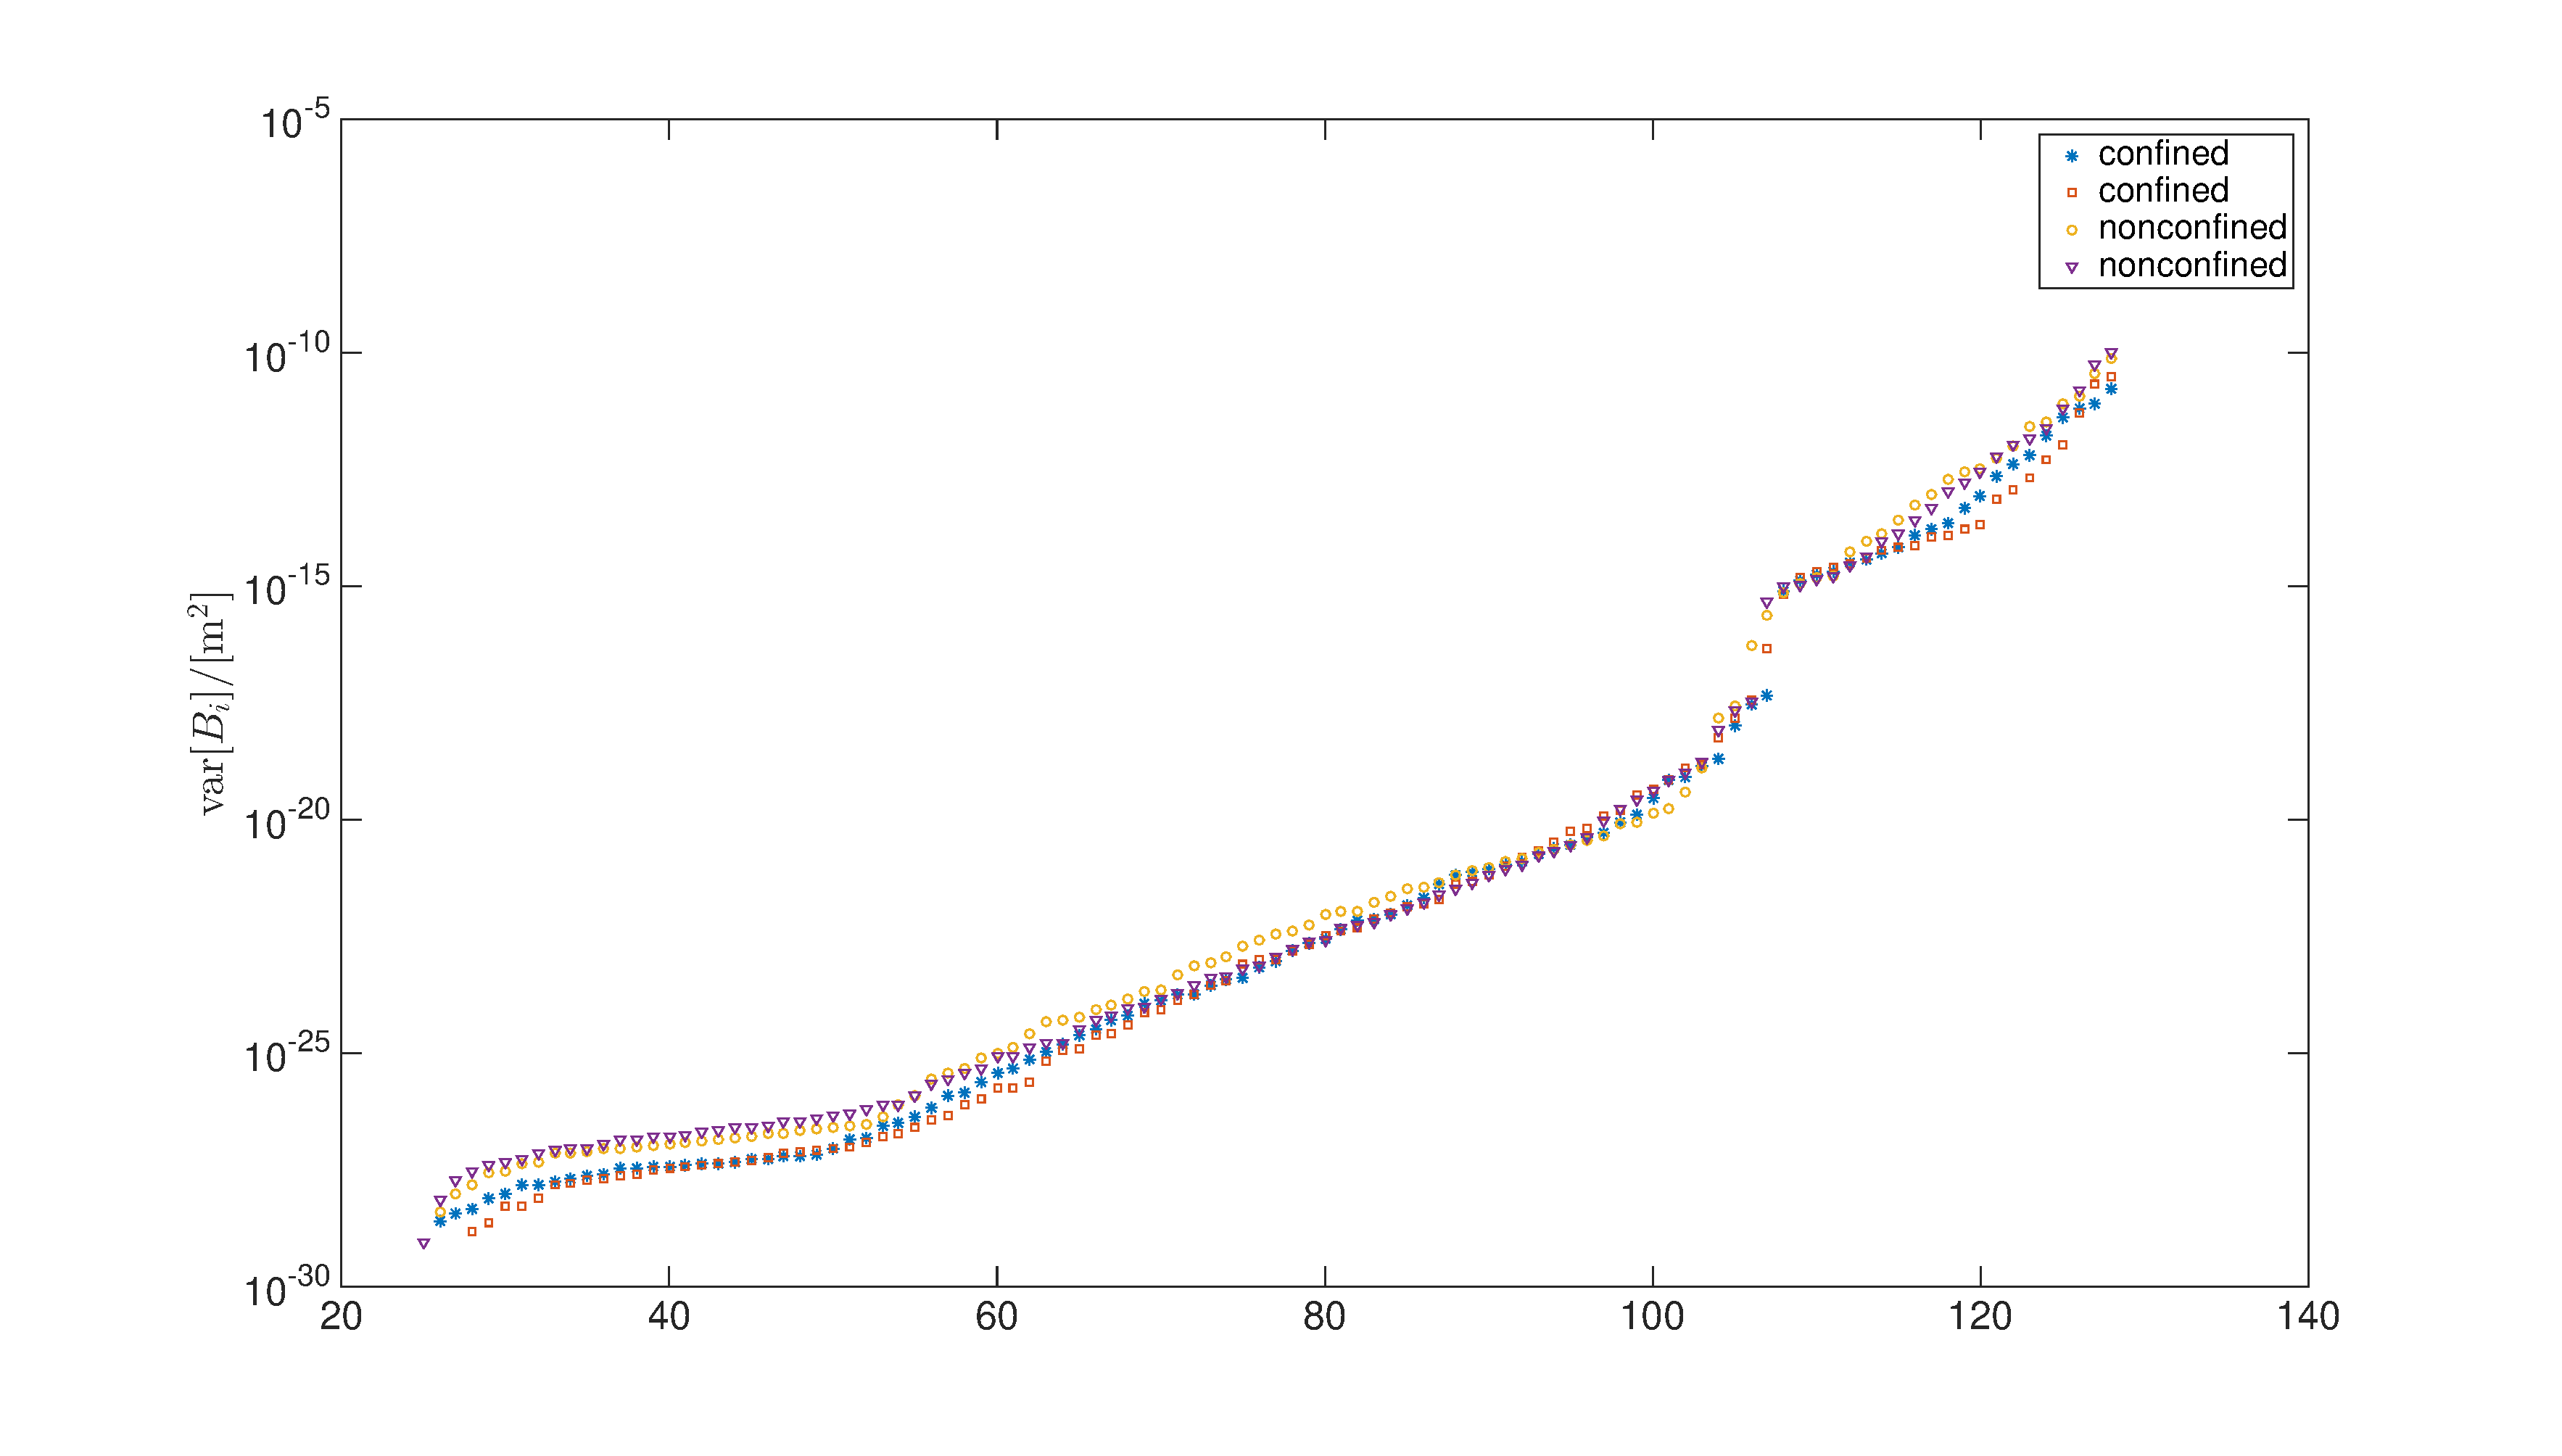
\includegraphics[width=.8\textwidth]{kovegenvarde.eps}
    \caption{Egenvärden till kovariansmatrisen bildad av avståndskomponenter till strängen relativt strängens jämviktsläge för fyra olika strängar. Det största egenvärdent ses vara ungefär $10^{16}$ ggr större än det minsta, vilket påvisar en signifikant skillnad i bidrag till rörelsen från egenmoderna. }
    \label{fig:kovegenvarde}
\end{figure}

\begin{figure}
    \centering
    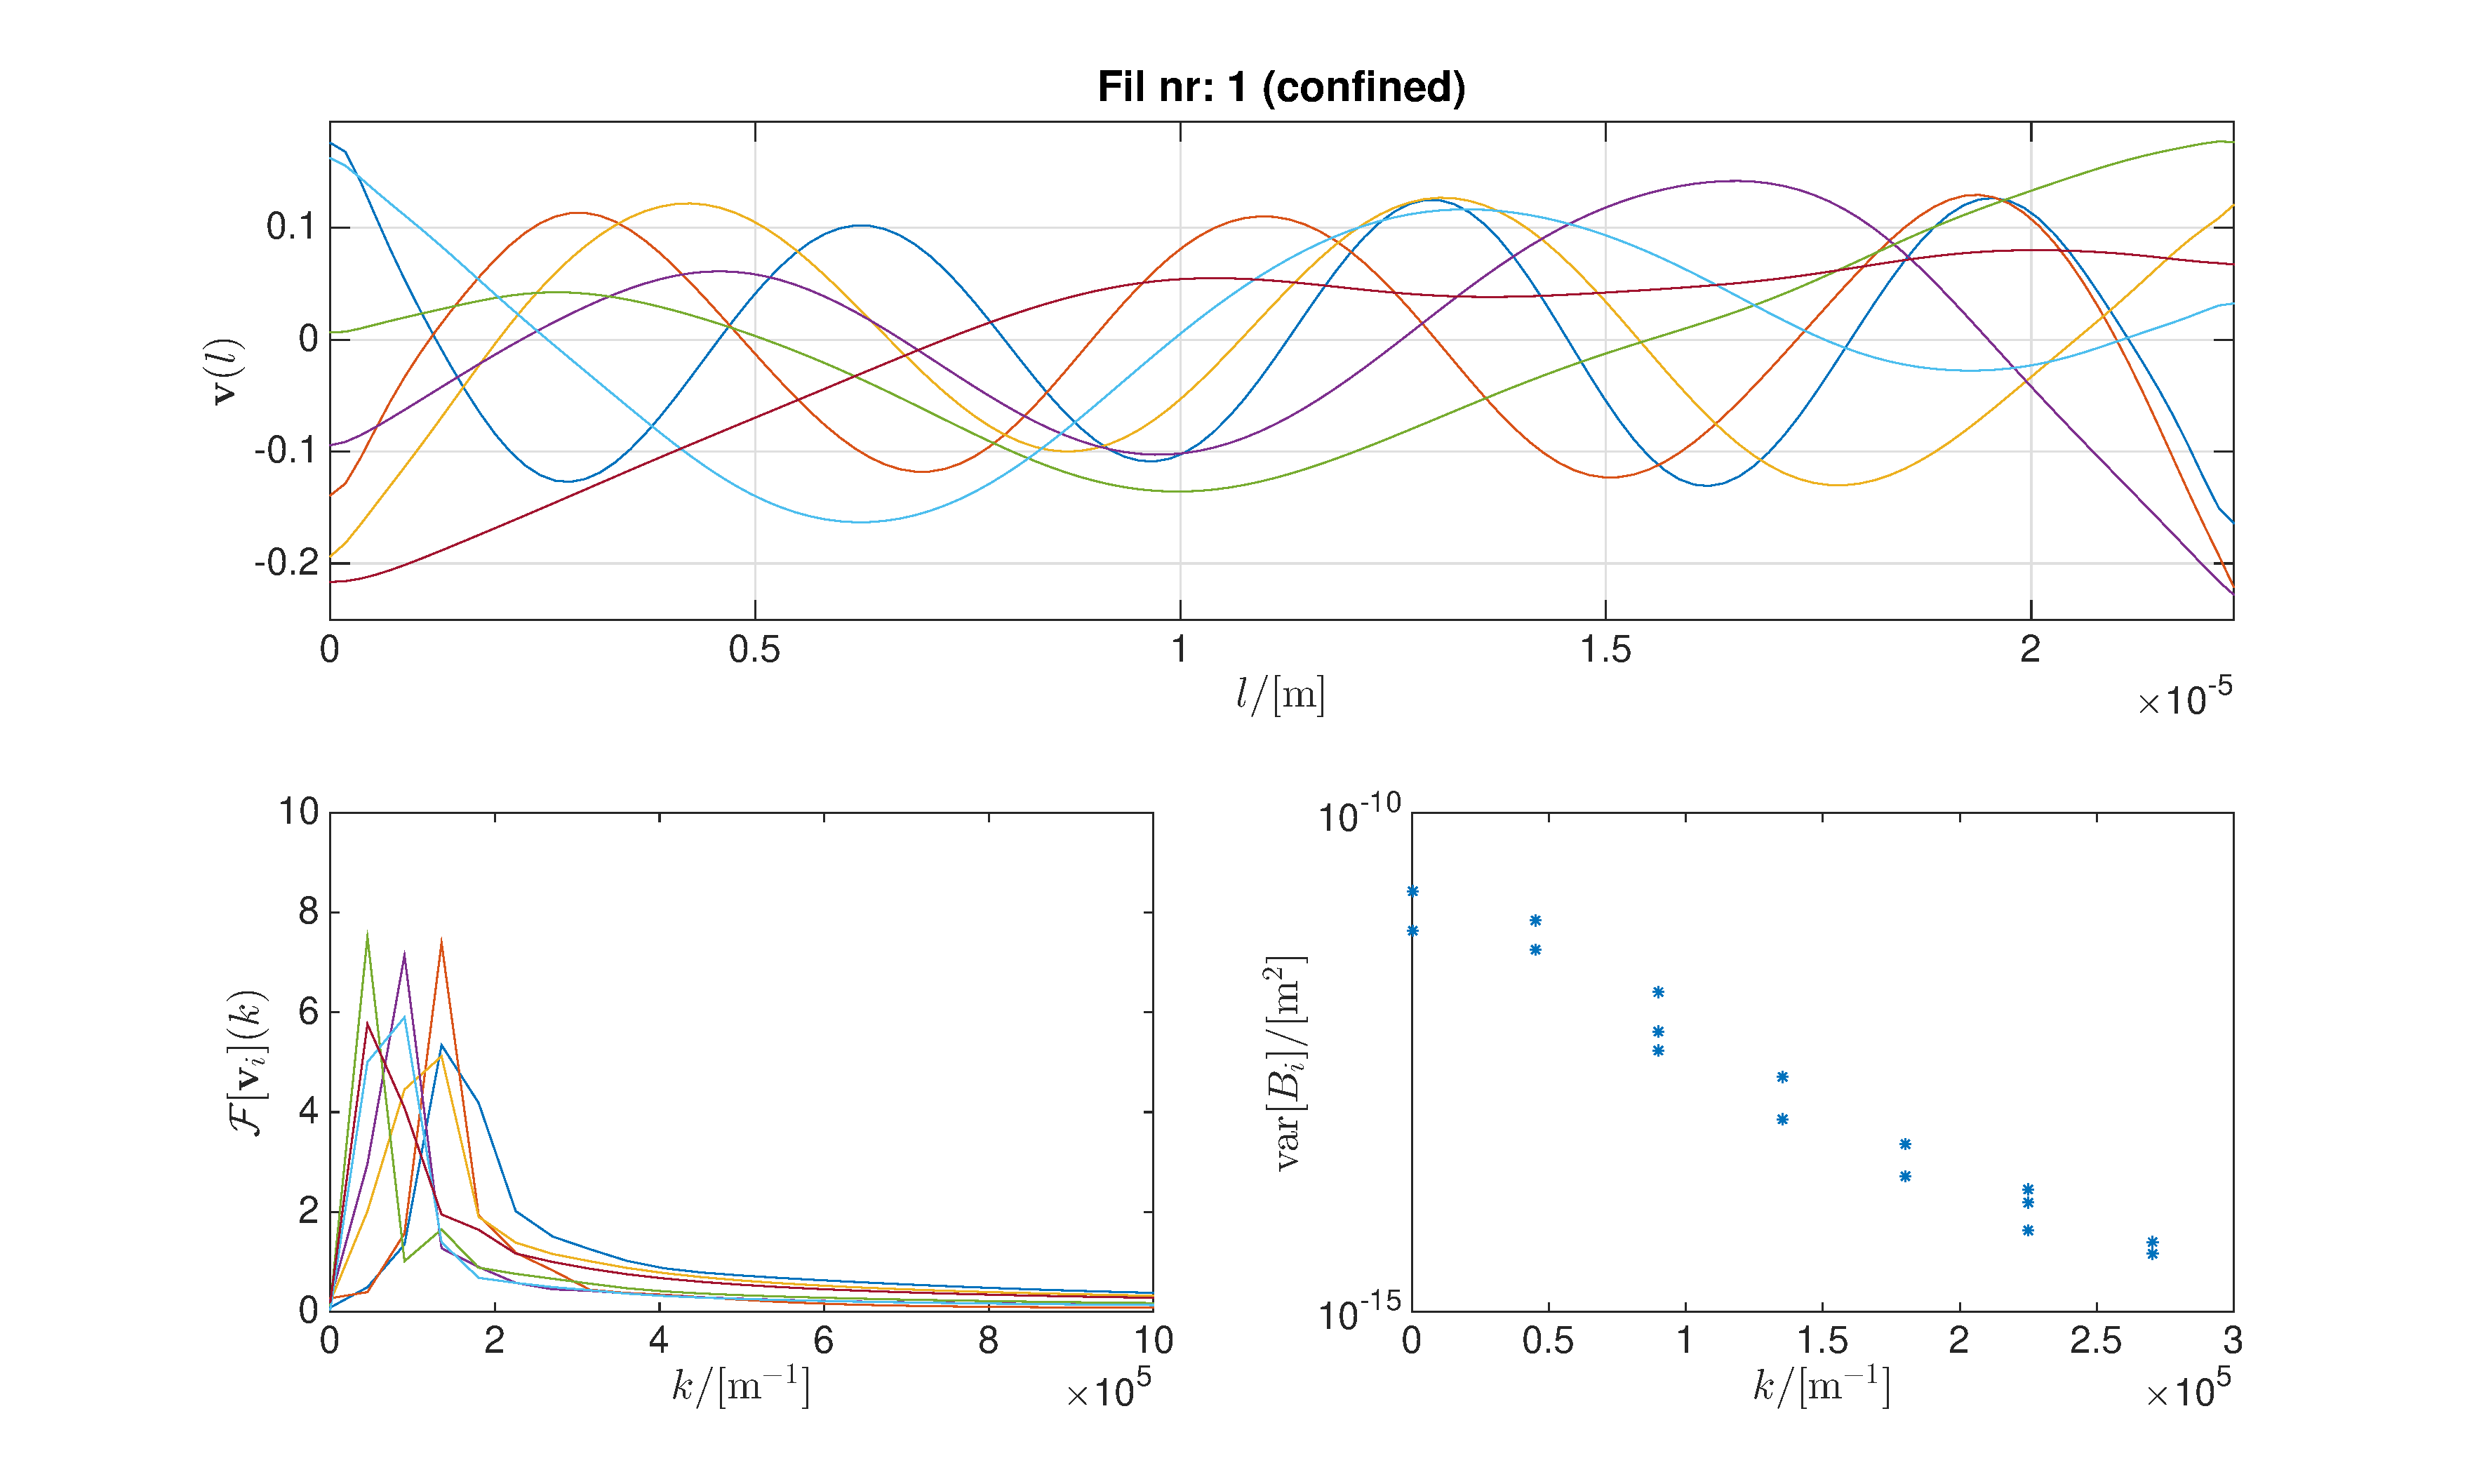
\includegraphics[width=\textwidth]{egenmoder.eps}
    \caption{Caption}
    \label{fig:egenmoder}
\end{figure}

%Resultat som kan tas med

%Motivera att jämviktsläge fanns
%Uppdelningen i egenmoder, olika relaxationstid
%Dispersionsrelation?
%Skillnad mellan confined och unconfined



\section{Diskussion}




%Bara en liten kodsnutt som behövs när man kompilerar lokalt
%%% Local Variables: 
%%% mode: latex
%%% TeX-master: "00main.tex"
%%% End: 